%
\documentclass[twoside]{article} % PREAMBLE

    \relax % Controls
        \newif\ifmarginprooflinks
        	\marginprooflinkstrue
        	% \marginprooflinksfalse

    \relax % Bibliography, etc
    	\usepackage[american]{babel}
    	\usepackage{csquotes}
    	\usepackage[backend=biber, style=authoryear]{biblatex}
    	\DeclareLanguageMapping{american}{american-apa}
    	% \usepackage[backend=biber,style=authoryear,hyperref=true]{biblatex}
    	\addbibresource{refs.bib}

    	\DeclareFieldFormat{citehyperref}{%
    	  \DeclareFieldAlias{bibhyperref}{noformat}% Avoid nested links
    	  \bibhyperref{#1}}

    	\DeclareFieldFormat{textcitehyperref}{%
    	  \DeclareFieldAlias{bibhyperref}{noformat}% Avoid nested links
    	  \bibhyperref{%
    	    #1%
    	    \ifbool{cbx:parens}
    	      {\bibcloseparen\global\boolfalse{cbx:parens}}
    	      {}}}

    	\savebibmacro{cite}
    	\savebibmacro{textcite}

    	\renewbibmacro*{cite}{%
    	  \printtext[citehyperref]{%
    	    \restorebibmacro{cite}%
    	    \usebibmacro{cite}}}

    	\renewbibmacro*{textcite}{%
    	  \ifboolexpr{
    	    ( not test {\iffieldundef{prenote}} and
    	      test {\ifnumequal{\value{citecount}}{1}} )
    	    or
    	    ( not test {\iffieldundef{postnote}} and
    	      test {\ifnumequal{\value{citecount}}{\value{citetotal}}} )
    	  }
    	    {\DeclareFieldAlias{textcitehyperref}{noformat}}
    	    {}%
    	  \printtext[textcitehyperref]{%
    	    \restorebibmacro{textcite}%
    	    \usebibmacro{textcite}}}

    	\DeclareCiteCommand{\brakcite}
    	  {\usebibmacro{prenote}}
    	  {\usebibmacro{citeindex}%
    	   \printtext[bibhyperref]{[\usebibmacro{cite}]}}
    	  {\multicitedelim}
    	  {\usebibmacro{postnote}}

    \relax % Standard Packages
        \usepackage[dvipsnames]{xcolor}
        % \usepackage[utf8]{inputenc}
        \usepackage{mathtools}
        \usepackage{amssymb}
    		\DeclareMathSymbol{\shortminus}{\mathbin}{AMSa}{"39}
        % \usepackage{parskip}
        % \usepackage{algorithm}
        \usepackage{bbm}
    	\usepackage{lmodern}
    	% \usepackage{times}
        \usepackage{faktor}
        % \usepackage{booktabs}
    	% \usepackage[margin=1in]{geometry}
        \usepackage{graphicx}
        \usepackage{scalerel}
        \usepackage{enumitem}
        \usepackage{nicefrac}\let\nf\nicefrac

        % \usepackage{color}
        %\usepackage{stmaryrd}
        \usepackage{hyperref} % Load before theorems...
            \hypersetup{colorlinks=true, linkcolor=blue!75!black, urlcolor=magenta, citecolor=green!50!black}

    \usepackage{tikz}
    	\usetikzlibrary{positioning,fit,calc, decorations, arrows, shapes, shapes.geometric}
    	\usetikzlibrary{cd}

    	%%%%%%%%%%%%
    	\tikzset{AmpRep/.style={ampersand replacement=\&}}
    	\tikzset{center base/.style={baseline={([yshift=-.8ex]current bounding box.center)}}}
    	\tikzset{paperfig/.style={center base,scale=0.9, every node/.style={transform shape}}}

    	% Node Stylings
    	\tikzset{dpadded/.style={rounded corners=2, inner sep=0.7em, draw, outer sep=0.3em, fill={black!50}, fill opacity=0.08, text opacity=1}}
    	\tikzset{dpad0/.style={outer sep=0.05em, inner sep=0.3em, draw=gray!75, rounded corners=4, fill=black!08, fill opacity=1, align=center}}
    	\tikzset{dpadinline/.style={outer sep=0.05em, inner sep=2.5pt, rounded corners=2.5pt, draw=gray!75, fill=black!08, fill opacity=1, align=center, font=\small}}

     	\tikzset{dpad/.style args={#1}{every matrix/.append style={nodes={dpadded, #1}}}}
    	\tikzset{light pad/.style={outer sep=0.2em, inner sep=0.5em, draw=gray!50}}

    	\tikzset{arr/.style={draw, ->, thick, shorten <=3pt, shorten >=3pt}}
    	\tikzset{arr0/.style={draw, ->, thick, shorten <=0pt, shorten >=0pt}}
    	\tikzset{arr1/.style={draw, ->, thick, shorten <=1pt, shorten >=1pt}}
    	\tikzset{arr2/.style={draw, ->, thick, shorten <=2pt, shorten >=2pt}}

    	\newcommand\cmergearr[5][]{
    		\draw[arr, #1, -] (#2) -- (#5) -- (#3);
    		\draw[arr, #1, shorten <=0] (#5) -- (#4);
    		}
    	\newcommand\mergearr[4][]{
    		\coordinate (center-#2#3#4) at (barycentric cs:#2=1,#3=1,#4=1.2);
    		\cmergearr[#1]{#2}{#3}{#4}{center-#2#3#4}
    		}
    	\newcommand\cunmergearr[5][]{
    		\draw[arr, #1, -, shorten >=0] (#2) -- (#5);
    		\draw[arr, #1, shorten <=0] (#5) -- (#3);
    		\draw[arr, #1, shorten <=0] (#5) -- (#4);
    		}
    	\newcommand\unmergearr[4][]{
    		\coordinate (center-#2#3#4) at (barycentric cs:#2=1.2,#3=1,#4=1);
    		\cunmergearr[#1]{#2}{#3}{#4}{center-#2#3#4}
    		}

    \usepackage{amsthm,thmtools} % Theorem Macros
    	\usepackage[noabbrev,nameinlink,capitalize]{cleveref}
        \theoremstyle{plain}
        \newtheorem{theorem}{Theorem}
    	\newtheorem{coro}{Corollary}[theorem]
        \newtheorem{prop}[theorem]{Proposition}
        \newtheorem{claim}{Claim}
        \newtheorem{remark}{Remark}
        \newtheorem{lemma}[theorem]{Lemma}
        \theoremstyle{definition}
        % \newtheorem{defn}{Definition}
        % \declaretheorem[name=Definition]{defn}
        \declaretheorem[name=Definition, qed=$\square$]{defn}
        \declaretheorem[name=Example, qed=$\triangle$]{example}

    	\crefname{defn}{Definition}{Definitions}
    	\crefname{prop}{Proposition}{Propositions}
        \crefname{issue}{Issue}{Issues}

    \relax %%%%%%%%% GENERAL MACROS %%%%%%%%
        \let\Horig\H
    	\let\H\relax
    	\DeclareMathOperator{\H}{\mathrm{H}} % Entropy
    	\DeclareMathOperator{\I}{\mathrm{I}} % Information
    	\DeclareMathOperator*{\Ex}{\mathbb{E}} % Expectation
    	\DeclareMathOperator*{\EX}{\scalebox{1.5}{$\mathbb{E}$}}

        \DeclarePairedDelimiter\bra{\langle}{\rvert}
        \DeclarePairedDelimiter\ket{\lvert}{\rangle}
        \DeclarePairedDelimiterX\braket[2]{\langle}{\rangle}{#1 \delimsize\vert #2}

        \newcommand{\mat}[1]{\mathbf{#1}}
        \DeclarePairedDelimiterX{\infdivx}[2]{(}{)}{%
    		#1\;\delimsize\|\;#2%
    	}
    	\newcommand{\thickD}{I\mkern-8muD}
    	\newcommand{\kldiv}{\thickD\infdivx}
    	\newcommand{\tto}{\rightarrow\mathrel{\mspace{-15mu}}\rightarrow}

    	\newcommand{\datadist}[1]{\Pr\nolimits_{#1}}
    	% \newcommand{\datadist}[1]{p_\text{data}}

    	\makeatletter
    	\newcommand{\subalign}[1]{%
    	  \vcenter{%
    	    \Let@ \restore@math@cr \default@tag
    	    \baselineskip\fontdimen10 \scriptfont\tw@
    	    \advance\baselineskip\fontdimen12 \scriptfont\tw@
    	    \lineskip\thr@@\fontdimen8 \scriptfont\thr@@
    	    \lineskiplimit\lineskip
    	    \ialign{\hfil$\m@th\scriptstyle##$&$\m@th\scriptstyle{}##$\hfil\crcr
    	      #1\crcr
    	    }%
    	  }%
    	}
    	\makeatother
    	\newcommand\numberthis{\addtocounter{equation}{1}\tag{\theequation}}

    \relax %%%%%%%%%   PDG  MACROS   %%%%%%%%
    	\newcommand{\ssub}[1]{_{\!_{#1}\!}}
    	% \newcommand{\bp}[1][L]{\mat{p}_{\!_{#1}\!}}
    	% \newcommand{\bP}[1][L]{\mat{P}_{\!_{#1}\!}}
    	\newcommand{\bp}[1][L]{\mat{p}\ssub{#1}}
    	\newcommand{\bP}[1][L]{\mat{P}\ssub{#1}}
    	\newcommand{\V}{\mathcal V}
    	\newcommand{\N}{\mathcal N}
    	\newcommand{\Ed}{\mathcal E}

        \newcommand{\balpha}{\boldsymbol\alpha}
        \newcommand{\bbeta}{\boldsymbol\beta}

    	\DeclareMathAlphabet{\mathdcal}{U}{dutchcal}{m}{n}
    	\DeclareMathAlphabet{\mathbdcal}{U}{dutchcal}{b}{n}
    	\newcommand{\dg}[1]{\mathbdcal{#1}}
    	\newcommand{\PDGof}[1]{{\dg M}_{#1}}
    	\newcommand{\UPDGof}[1]{{\dg N}_{#1}}
    	\newcommand\VFE{\mathit{V\mkern-4mu F\mkern-4.5mu E}}

    	\newcommand\Inc{\mathit{Inc}}
    	\newcommand{\IDef}[1]{\mathit{IDef}_{\!#1}}
    	% \newcommand{\ed}[3]{%
    	% 	\mathchoice%
    	% 	{#2\overset{\smash{\mskip-5mu\raisebox{-3pt}{${#1}$}}}{\xrightarrow{\hphantom{\scriptstyle {#1}}}} #3} %display style
    	% 	{#2\overset{\smash{\mskip-5mu\raisebox{-3pt}{$\scriptstyle {#1}$}}}{\xrightarrow{\hphantom{\scriptstyle {#1}}}} #3}% text style
    	% 	{#2\overset{\smash{\mskip-5mu\raisebox{-3pt}{$\scriptscriptstyle {#1}$}}}{\xrightarrow{\hphantom{\scriptscriptstyle {#1}}}} #3} %script style
    	% 	{#2\overset{\smash{\mskip-5mu\raisebox{-3pt}{$\scriptscriptstyle {#1}$}}}{\xrightarrow{\hphantom{\scriptscriptstyle {#1}}}} #3}} %scriptscriptstyle
    	\newcommand{\ed}[3]{#2%
    	  \overset{\smash{\mskip-5mu\raisebox{-1pt}{$\scriptscriptstyle
    	        #1$}}}{\rightarrow} #3}

        \newcommand{\nhphantom}[2]{\sbox0{\kern-2%
    		\nulldelimiterspace$\left.\delimsize#1\vphantom{#2}\right.$}\hspace{-.97\wd0}}
    		% \nulldelimiterspace$\left.\delimsize#1%
    		% \vrule depth\dp#2 height \ht#2 width0pt\right.$}\hspace{-.97\wd0}}
    	\makeatletter
    	\newsavebox{\abcmycontentbox}
    	\newcommand\DeclareDoubleDelim[5]{
    	    \DeclarePairedDelimiterXPP{#1}[1]%
    			{% box must be saved in this pre code
    				\sbox{\abcmycontentbox}{\ensuremath{##1}}%
    			}{#2}{#5}{}%
    		    %%% Correct spacing, but doesn't work with externalize.
    			% {\nhphantom{#3}{##1}\hspace{1.2pt}\delimsize#3\mathopen{}##1\mathclose{}\delimsize#4\hspace{1.2pt}\nhphantom{#4}{##1}}
    			%%% Fast, but wrong spacing.
    			% {\nhphantom{#3}{~}\hspace{1.2pt}\delimsize#3\mathopen{}##1\mathclose{}\delimsize#4\hspace{1.2pt}\nhphantom{#4}{~}}
    			%%% with savebox.
    		    {%
    				\nhphantom{#3}{\usebox\abcmycontentbox}%
    				\hspace{1.2pt} \delimsize#3%
    				\mathopen{}\usebox{\abcmycontentbox}\mathclose{}%
    				\delimsize#4\hspace{1.2pt}%
    				\nhphantom{#4}{\usebox\abcmycontentbox}%
    			}%
    	}
    	\makeatother
    	\DeclareDoubleDelim
    		\SD\{\{\}\}
    	\DeclareDoubleDelim
    		\bbr[[]]
    	% \DeclareDoubleDelim
    	% 	\aar\langle\langle\rangle\rangle
    	\makeatletter
    	\newsavebox{\aar@content}
    	\newcommand\aar{\@ifstar\aar@one@star\aar@plain}
    	\newcommand\aar@one@star{\@ifstar\aar@resize{\aar@plain*}}
    	\newcommand\aar@resize[1]{\sbox{\aar@content}{#1}\scaleleftright[3.8ex]
    		{\Biggl\langle\!\!\!\!\Biggl\langle}{\usebox{\aar@content}}
    		{\Biggr\rangle\!\!\!\!\Biggr\rangle}}
    	\DeclareDoubleDelim
    		\aar@plain\langle\langle\rangle\rangle
    	\makeatother


    	% \DeclarePairedDelimiterX{\aar}[1]{\langle}{\rangle}
    	% 	{\nhphantom{\langle}{#1}\hspace{1.2pt}\delimsize\langle\mathopen{}#1\mathclose{}\delimsize\rangle\hspace{1.2pt}\nhphantom{\rangle}{#1}}

    \relax %%%%% restatables and links
    	% \usepackage{xstring} % for expandarg
    	\usepackage{xpatch}
    	\makeatletter
    	\xpatchcmd{\thmt@restatable}% Edit \thmt@restatable
    	   {\csname #2\@xa\endcsname\ifx\@nx#1\@nx\else[{#1}]\fi}% Replace this code
    	   % {\ifthmt@thisistheone\csname #2\@xa\endcsname\typeout{oiii[#1;#2\@xa;#3;\csname thmt@stored@#3\endcsname]}\ifx\@nx#1\@nx\else[#1]\fi\else\csname #2\@xa\endcsname\fi}% with this code
    	   {\ifthmt@thisistheone\csname #2\@xa\endcsname\ifx\@nx#1\@nx\else[{#1}]\fi
    	   \else\fi}
    	   {}{\typeout{FIRST PATCH TO THM RESTATE FAILED}} % execute on success/failure
    	\xpatchcmd{\thmt@restatable}% A second edit to \thmt@restatable
    	   {\csname end#2\endcsname}
    	   {\ifthmt@thisistheone\csname end#2\endcsname\else\fi}
    	   {}{\typeout{FAILED SECOND THMT RESTATE PATCH}}

    	% \def\onlyaftercolon#1:#2{#2}
    	\newcommand{\recall}[1]{\medskip\par\noindent{\bf \Cref{thmt@@#1}.} \begingroup\em \noindent
    	   \expandafter\csname#1\endcsname* \endgroup\par\smallskip}

       	\setlength\marginparwidth{1.55cm}
    	\newenvironment{linked}[3][]{%
    		\def\linkedproof{#3}%
    		\def\linkedtype{#2}%
    		% \reversemarginpar
    		% \marginpar{%
    		% \vspace{1.1em}
    		% % \hspace{2em}
    		% 	% \raggedleft
    		% 	\raggedright
    		% 	\hyperref[proof:\linkedproof]{%
    		% 	\color{blue!50!white}
    		% 	\scaleleftright{$\Big[$}{\,{\small\raggedleft\tt\begin{tabular}{@{}c@{}} proof of \\\linkedtype~\ref*{\linkedtype:\linkedproof}\end{tabular}}\,}{$\Big]$}}
    		% 	}%
            % \restatable[#1]{#2}{#2:#3}\label{#2:#3}%
    		\ifmarginprooflinks
    		\marginpar{%
    			% \vspace{-3em}% %% for bottom
    			\vspace{1.5em}
    			\centering%
    			\hyperref[proof:\linkedproof]{%
                % \hyperref[proof:#3]{
    			\color{blue!30!white}%
    			\scaleleftright{$\Big[$}{\,\mbox{\footnotesize\centering\tt\begin{tabular}{@{}c@{}}
    				% proof of \\\,\linkedtype~\ref*{\linkedtype:\linkedproof}
    				link to\\[-0.15em]
    				proof
    			\end{tabular}}\,}{$\Big]$}}~
    			}%
    		\fi
            \restatable[#1]{#2}{#2:#3}\label{#2:#3}%
            }%
    		{\endrestatable%
    		}
    	\makeatother
    		\newcounter{proofcntr}
    		\newenvironment{lproof}{\begin{proof}\refstepcounter{proofcntr}}{\end{proof}}

    		\usepackage{cancel}
    		\newcommand{\Cancel}[2][black]{{\color{#1}\cancel{\color{black}#2}}}

    		\usepackage{tcolorbox}
    		\tcbuselibrary{most}
    		\tcolorboxenvironment{lproof}{
    			% fonttitle=\bfseries,
    			% top=0.5em,
    			enhanced,
    			parbox=false,
    			boxrule=0pt,
    			frame hidden,
    			borderline west={4pt}{0pt}{blue!20!black!40!white},
    			% coltext={blue!20!black!60!white},
    			colback={blue!20!black!05!white},
    			sharp corners,
    			breakable,
    			% bottomsep at break=4cm,
    			% enlarge bottom at break by=-4cm,
    			% topsep at break=3cm,
    			% enlarge top at break by=-3cm
    		}
    		% \usepackage[framemethod=TikZ]{mdframed}
    		% \surroundwithmdframed[ % lproof
    		% 	   topline=false,
    		% 	   linewidth=3pt,
    		% 	   linecolor=gray!20!white,
    		% 	   rightline=false,
    		% 	   bottomline=false,
    		% 	   leftmargin=0pt,
    		% 	   % innerleftmargin=5pt,
    		% 	   skipabove=\medskipamount,
    		% 	   skipbelow=\medskipamount
    		% 	]{lproof}
    	%oli16: The extra space was because there was extra space in the paragraph, not
    	%because this length was too big. By breaking arrays, everything will be better.
    	\newcommand{\begthm}[3][]{\begin{#2}[{name=#1},restate=#3,label=#3]}

    \relax %TODOs and footnotes
        \newcommand{\TODO}[1][INCOMPLETE]{{\centering\Large\color{red}$\langle$~\texttt{#1}~$\rangle$\par}}
        \newcommand{\dfootnote}[1]{%
            \let\oldthefootnote=\thefootnote%
            % \addtocounter{footnote}{-1}%
    		\setcounter{footnote}{999}
            \renewcommand{\thefootnote}{\textdagger}%
            \footnote{#1}%
            \let\thefootnote=\oldthefootnote%
        }
    	\newcommand{\dfootnotemark}{
    		\footnotemark[999]
    	}

% \twocolumn
\setlength\parskip{1ex}

\usepackage{parskip}
\usepackage[margin=1in]{geometry}

\begin{document}
    What do the confidence parameters $\balpha$ and $\bbeta$ mean?
    I will give a number of different answers to this question.


% \section{}
% What matters is the values of $\beta$ relative to one another

\section{Trust and Dominance}\label{sec:trust-dominance}
    % One simple solution to \cref{issue:conflictconfidence} is to slightly alter the names and interpretations of the parameters $\balpha, \bbeta$, so as to clarify their differences and their roles in the model.
    % Indeed, even if we do provide an explanation of the parameters in terms of more basala
    %
    % if we are to retain the PDG semantics the way that they currently work.
    %
    % I propose calling $\bbeta$ ``trust'', and $\balpha$ ``dominance''.


    \subsection{Trust}

    We have said before that what's important is not the absolute value of $\beta_L$, but rather the values of $\beta$ relative to one another (and to $\gamma$).



    \textbf{Measuring Trust.}
    % We measure trust in $\bbeta$ disutility per error.
    % Each unit of discrepency a highly trusted information and reality is painful (the pain of betrayed trust).
    One way of measuring trust ($\beta$) is in units of disutility per error: errors in highly trusted information are painful, while it violations of untrusted information do not cause pain.
    Recall that utilities behave identically when scaled uniformly by a positive constant.
    So, units of disutils per error reflect the fact that scaling every $\beta$ (and $\gamma$) by a positive constant $k$ results in qualitatively identical semantics: whether one distribution scores higher than another does not depend on this choice of scale.

    To be a little more careful, we may want to regard beliefs (probabilistic information and confidence) as separate from utility.
    % In this interperetation, the mathematics is the same, but rather than utility, we now turn to the (higher order) \emph{negative log likelihood} (NLL), which we submit is an analog of disutility for beliefs.
    To this end, we consider an analog of disutility for beliefs --- that is, an ``unlikeliness'' function $V(\mu)$ on joint distributions, which takes larger values the less likely we think $\mu$ is. The scoring function of a PDG is an example of such a function.
    Now, given such a function $V(\mu)$ and some constant $k$, consider the following transformation of it:
    \[ \Pr(\mu) \propto \exp( -k V(\mu)).\]
    This way of turning ``unlikeliness/badness'' into probabilitiy distributions is standard and well-justified in statistical mechanics, where it is known as a Boltzman distribution.
    This transformation is invertable. Given the higher order probability $\Pr(\mu)$, we can write $V(\mu) = - k \log \Pr(\mu) + C$ for some constant $C$.  Note that as $k \to \infty$, $\Pr(\mu)$ becomes concentrated entirely on the minimizer(s) of $V$, so if $V$ has a unique minimum, $\Pr$ becomes a point mass on the least-bad distribution $\mu^*$. Note also that the $C$ is destroyed when we normalize the distribution $\Pr$, and scaling of $V(\mu)$ by a positive constant doesn't affect the limit as $k \to \infty$ --- so the constants $C$ and $k$ absorb positive affine transformations, which is one reason we liken it to a utility.

    In any case, if we're interested in modeling a higher-order distribution $\Pr(\mu)$; we have now seen that it suffices to model $V(\mu)$ instead, since it contains the same information.

    With this context in mind, let's return to $\beta$.
    % We have a collection of cpds, each of which has confidence.
    % We're trying to build $V(\mu)$, from a collection of cpds and confidences.
    % $\beta_L$
    In the context of a PDG, the modeler has given a collection of cpds and a value indicating how much to trust each one.
    Given only this information, it seems natural that distributions $\mu$ that are ``further away'' from a cpd should be less likely, and more so if the cpd is highly trusted. So:
    \begin{enumerate}
        \item A large value of $\beta_L$, which states that the cpd $p \ssub L(Y|X)$ is highly trusted, means that distributions $\mu$ that deviate from it significantly are very unlikely.
        \item A value of $\beta_L = 0$ indicates that the associated cpd $p\ssub L(Y|X)$ is \emph{un}trusted should not influence the calculus, and may as well be replaced with another.
        \item Negative values of $\beta_L$ indicate that being close to the cpd $p\ssub L(Y|X)$ makes a distribution $\mu$ \emph{less} likely, indicating that $p$ is actively \emph{dis}trusted.
    \end{enumerate}

    In some sense, $\beta_L$ is a curvature of the higher order probability distribution $\Pr(\mu)$
    To reiterate, the absolute scale doesn't matter; what matters is the values of $\beta$ relative to one another. This begs the following question:

    % We can make this more concrete once we decide how to measure this divergence between $\mu$ and a given cpd. The PDG formalism uses relative entropy, in which case the units of
    %
    % and weights $\beta$, which define an unlikeliness by
    % \[ V(\mu) := \Inc(\mu) = \sum_L \mathrm \]


    % \textbf{Beta as a dual vector.}
    \textbf{What does it mean to say that $\beta_p = 2 \beta_{q}$?}
    That a cpd $p$ is twice as trusted as a cpd $q$?
    It means that

    \begin{itemize}
        \item If $p$ and $q$ turn out to be in conflict, so that we have to choose between them, we put twice as much stock in $p$ as in $q$.
        \item If both $p$ and $q$ turn out to be equally wrong, the pain of betrayal after having trusted $p$ is twice that of the betrayal of $q$.
    \end{itemize}

    While these explanations are intuitive on some level, they are not very concrete.
    In the first case, we have to explain how to measure ``stock''; in the second, we have to explain how to measure ``pain of betrayal''.  The choice of measure here, which is necessary to make this concrete, turns out to essentially be the same as the choice of distance measure between probability distributions in PDG semantics.

    To illustrate, let $\thickD$ be some abstract measure of divergence.
    With the data of the PDG, consider the following estimate of the unlikeliness, as a linear combination of the basis functions $\{ \kldiv-{p_L}$ for $L \in \Ed$:
    \[
        V(\mu) := \Inc(\mu) = \sum_{\ed LXY} \beta_L \kldiv{\mu}{p},
    \]
    and $\bbeta$ describes the cofficients of the basis functions.
    So, we may also think of $\beta$ as the linear regression coefficients of some internal model of $V(X)$, with respect to each of the cpds in the PDG.

    Trust may then be described in units of unlikeliness ($V(\mu)$) per unit of divergence.  In the standard presentation of PDGs, $\thickD$ is relative entropy (measured in bits), in which case trust is measured in per unlikeliness (which you could measure in dollars or euros with a betting game) per bit of error.
    So, what does it mean to say that $\beta_p = 2 \beta_{q}$?
    It means that, all else being equal, a distribution $\mu$ is regarded as twice as unlikely per unit of distance from $p$ as it is per unit distance from $q$.


    \textbf{Relationships to Other Quantities.}
    This notion of trust is not entirely new; it has deep connections to a number of other very standard concepts throughout mathematics.

    \begin{enumerate}
        \item \textbf{Regression Coefficients.} [TODO]

        \item \textbf{Dual Vectors in Support Vector Machines.} This is arguably an application of the previous point. A support vector machine describes a hypothesis as a linear combinations of some of the training examples (the ``support vectors''). The standard

        \item \textbf{Coefficient of Boltzman Rationality.} [TODO]

        \item \textbf{Thermodynamic Coldness (inverse temperature).} [TODO]

    \end{enumerate}



    \textbf{So, how should one choose values of $\beta$?}
    We will give a few different approaches, but ultimately, $\beta$ is the primitive of a PDG.
    We will describe a way of setting $\beta$ given a higer order probability distribution $\Pr(\mu)$ over joint distributions $\mu$ --- but if you truly had such beliefs, you should have encoded them directly into your PDG.
    If you have a probability that the information is trustworthy, you should encode that directly as well.

    That said, one can derive $\beta$ as the optimal linear regression coefficients with respect to the basis Distance functions.
    (although this is a computationally expensive and a sub-optimal modling choice if you already have $\Pr(\mu)$).


    % Of course, every edge of any encoding requires a $\beta$; with a PDG, you may specify





    \textbf{Some additional thoughts on the word ``trust''.}
    \begin{itemize}
        \item It is a close synonym of ``confidence'', which was the original presentation.

        \item It also has a standard meaning in terms of capital: a trust is in some sense a financial asset, often in the form of a portfolio of investments optimized for stability. Its magnitude can be measured in dollars.
        Furthermore, an investment portfolio in some sense reflects probabilistic beliefs (they are bets about what is likely to go up and down in value), and because the point is stability, the capital is concentrated in beliefs one has high confidence in.

        \item Interpreting $\beta$ as ``pain of betrayal arising from inaccuracy'' gives us an intuitive meaning if it is negative: the vindication of seeing information you actively \emph{distrust} proven wrong.
    \end{itemize}





    \subsection{Dominance}
    % Dominance, on the other hand, is unitless; it is specified relative to
    % Dominance, on the other hand, is relative to
    While we have described $\beta_L$ as trust, or ``quantitative confidence'' in the cpd $p_L$,
    $\alpha_L$ is its qualitative analog: ``qualitative confidence'' in the functional relationship ``$Y$ determines X'' implicit in the edge $\ed LXY$.

    First, the techincal way in which $\balpha$ is analogous to $\bbeta$.
    Just as $\bbeta$ can be thought of as the optimal regression coefficients for a set of divergence basis functions, $\balpha$ are the optimal coefficients for additional basis functions: the uncertainties along each edge.


    \textbf{How to set $\balpha$}

    [TODO]

    \begin{center}
        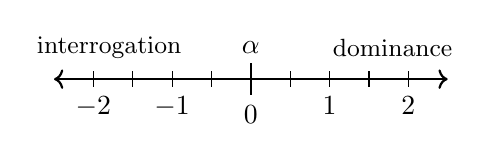
\begin{tikzpicture}
            \draw[thick, <->] (-2.5,0) -- (2.5, 0);
            \foreach \x in {-2.0, -1.5, ..., 2.0} {
                \draw[thin] (\x, 0.1) -- (\x,-0.1);
            }
            \foreach \x in {-2, -1, 1, 2} {
                \draw[thin] (\x, 0.1) -- (\x,-0.1) node[below]{$\x$};
            }
            \draw[thick] (0,0.2) -- (0,-0.2) node[below] {$0$};
            \node at  ( 0 , 0.4) {$\alpha$};
            \node[font=\small] at ( 1.8, 0.4) {dominance};
            \node[font=\small] at (-1.8, 0.4) {interrogation};

        \end{tikzpicture}
    \end{center}

    % \TODO
    % Interrogative strength.

\section{The System}
    Let $\mathcal A$ be a collection of agents, each with certain beleifs.


\subsection{A Hamiltonian}
Let $\ket\psi := \beta  + i\alpha$.
\[
    \H \ket\psi :=
\]

\section{The Betting Game}
    Suppose there are two agents, that are aware of the same set of concepts, corresponding to the variables $\mathbf X = (\N, \V)$.
    Agent 1's beliefs are given by the PDG
    % $\dg M_1 = (\N, \Ed^1, \V, \mat p^1, \balpha^1, \bbeta^1)$,
    $\dg M_1 = (\mat X, \Ed^1,\balpha^1, \mat p^1, \bbeta^1)$,
    while agent 2's beliefs are given by the PDG
    % $\dg M_2 = (\N, \Ed^2, \V, \mat p^2, \balpha^2, \bbeta^2)$.
    $\dg M_2 = (\mat X, \Ed^2,\balpha^2, \mat p^2, \bbeta^2)$.

    Recall that for any cpd $\bp(Y|X)$, the optimal code for communicating $Y$ from samples of $X$ have length $\I^{Y|X}_{\bp} := - \log {\bp(Y|X)}$.

    First, you bet

    Now, suppose that in reality, variables are distributed according to some joint distribution $\rho(\mathbf X)$.



\appendix



\section{}

% \subsubsection{On Subjectivenss of Utility: Is it a Problem?}
% \label{disutility:subjective}
%
% The whole point of (expected) utility is that you can use it to numerically compare outcomes in goodness. It comes with the
%
% It is true that utility is not comparable across different people, but really the point is that the pain of betrayal of one belief versus another can be traded off.
% The actual values of the numbers can be different and you can have an equivalent model\footnote{for instance, one can always double $\bbeta$ and $\gamma$ to double the scoring function, resulting in the same optima and qualitative features}.




\section{Scraps}

\begin{align*}
   \bbr{\dg M}_\gamma(\mu) =
   \Ex_{\mu}\left[
       \braket[\Big]{\bbeta^{\dg M}}{\I_{\dg M}- \I_{\mu}}
       + \gamma
       \braket[\Big]{\balpha^{\dg M} - \balpha^{\mu}} {\I_\mu - \I_\lambda}
   \right]
\end{align*}

\[
% \bbr[\Big]{(\rho, \gamma) \models \dg M_1 \to \dg M_2 }  =
\mathcal U_{(\rho, \gamma)}\Big(\dg M_2 \gets \dg M_1 \Big)  =
   % \Ex_{\rho}\left[
   %     \braket[\Big]{\bbeta^{\dg M_1}}{\I_{\dg M_1}- \I_{\dg M_2}}
   %     + \gamma
   %     \braket[\Big]{\balpha^{\dg M_1} - \balpha^{\dg M_2}} {\I_\rho - \I_\lambda}
   % \right]
   \Ex_{\rho}\left[
       \braket[\Big]{\bbeta^{1}}{\I_{\dg M_1}- \I_{\dg M_2}}
       + \gamma
       \braket[\Big]{\balpha^{1} - \balpha^{2}} {\I_\rho + (\mathbbm1[\alpha^2 \!<\!0] - \mathbbm1[\alpha^1\!<\!0])\I_\lambda}
   \right]
\]

Or, without the strangeness with the sign of $\alpha$:
\[
% \bbr[\Big]{(\rho, \gamma) \models \dg M_1 \to \dg M_2 }  =
\mathcal U_{(\rho, \gamma)}\Big(\dg M_2 \gets \dg M_1 \Big)  =
   % \Ex_{\rho}\left[
   %     \braket[\Big]{\bbeta^{\dg M_1}}{\I_{\dg M_1}- \I_{\dg M_2}}
   %     + \gamma
   %     \braket[\Big]{\balpha^{\dg M_1} - \balpha^{\dg M_2}} {\I_\rho - \I_\lambda}
   % \right]
   \Ex_{\rho}\left[
       \braket[\Big]{\bbeta^{1}}{\I_{\dg M_1}- \I_{\dg M_2}}
       + \gamma
       \braket[\Big]{\balpha^{1} - \balpha^{2}} {\I_\rho - \I_\lambda}
   \right]
\]


\end{document}
